\setcounter{definition}{0} \setcounter{property}{0} \setcounter{claim}{0} \setcounter{fact}{0} \setcounter{corollary}{0} \setcounter{figure}{0}
\section{Convex Hull}

\subsection*{Definitions}

\begin{definition}[Convex Hull]
Let $P = \{p_1, p_2, \cdots, p_n\}$ be a set of points on 2D plane, each of which is represented as $p_i = (x_i, y_i)$.
The \emph{convex hull} of $P$, denoted as $CH(P)$, is defined as the smallest, convex polygon that includes all points in $P$.
\end{definition}

A convex hull is usually represented as the list of vertices~(which is subset
of $P$) of the polygon in counter-clockwise order. Such list 
is circular, and it's equivalent to shifting any number of vertices.
If a point $p\in P$ is one of the vertices of the convex hull of $P$,
we usually say that $p$ is \emph{on} the convex hull, and denote it as $p\in CH(P)$.

\begin{figure}[h!]
\centering{

\tikzset{every picture/.style={line width=0.75pt}} %set default line width to 0.75pt        

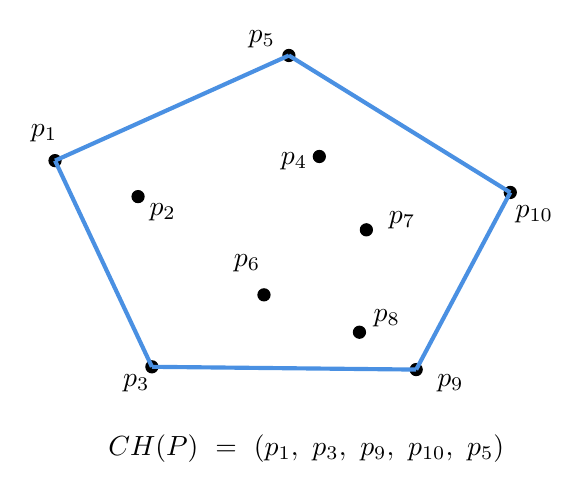
\begin{tikzpicture}[x=0.5pt,y=0.5pt,yscale=-1,xscale=1]
%uncomment if require: \path (0,420); %set diagram left start at 0, and has height of 420

%Flowchart: Connector [id:dp05090347480351787] 
\draw  [fill={rgb, 255:red, 0; green, 0; blue, 0 }  ,fill opacity=1 ] (57,162) .. controls (57,159.58) and (58.96,157.62) .. (61.38,157.62) .. controls (63.79,157.62) and (65.75,159.58) .. (65.75,162) .. controls (65.75,164.42) and (63.79,166.38) .. (61.38,166.38) .. controls (58.96,166.38) and (57,164.42) .. (57,162) -- cycle ;
%Flowchart: Connector [id:dp3291568735294871] 
\draw  [fill={rgb, 255:red, 0; green, 0; blue, 0 }  ,fill opacity=1 ] (226,86) .. controls (226,83.58) and (227.96,81.62) .. (230.38,81.62) .. controls (232.79,81.62) and (234.75,83.58) .. (234.75,86) .. controls (234.75,88.42) and (232.79,90.38) .. (230.38,90.38) .. controls (227.96,90.38) and (226,88.42) .. (226,86) -- cycle ;
%Flowchart: Connector [id:dp6621594719883535] 
\draw  [fill={rgb, 255:red, 0; green, 0; blue, 0 }  ,fill opacity=1 ] (318,313) .. controls (318,310.58) and (319.96,308.62) .. (322.38,308.62) .. controls (324.79,308.62) and (326.75,310.58) .. (326.75,313) .. controls (326.75,315.42) and (324.79,317.38) .. (322.38,317.38) .. controls (319.96,317.38) and (318,315.42) .. (318,313) -- cycle ;
%Flowchart: Connector [id:dp25920829224973985] 
\draw  [fill={rgb, 255:red, 0; green, 0; blue, 0 }  ,fill opacity=1 ] (127,311) .. controls (127,308.58) and (128.96,306.62) .. (131.38,306.62) .. controls (133.79,306.62) and (135.75,308.58) .. (135.75,311) .. controls (135.75,313.42) and (133.79,315.38) .. (131.38,315.38) .. controls (128.96,315.38) and (127,313.42) .. (127,311) -- cycle ;
%Flowchart: Connector [id:dp02220382507011076] 
\draw  [fill={rgb, 255:red, 0; green, 0; blue, 0 }  ,fill opacity=1 ] (117,188) .. controls (117,185.58) and (118.96,183.62) .. (121.38,183.62) .. controls (123.79,183.62) and (125.75,185.58) .. (125.75,188) .. controls (125.75,190.42) and (123.79,192.38) .. (121.38,192.38) .. controls (118.96,192.38) and (117,190.42) .. (117,188) -- cycle ;
%Flowchart: Connector [id:dp5073811152902622] 
\draw  [fill={rgb, 255:red, 0; green, 0; blue, 0 }  ,fill opacity=1 ] (386,185) .. controls (386,182.58) and (387.96,180.62) .. (390.38,180.62) .. controls (392.79,180.62) and (394.75,182.58) .. (394.75,185) .. controls (394.75,187.42) and (392.79,189.38) .. (390.38,189.38) .. controls (387.96,189.38) and (386,187.42) .. (386,185) -- cycle ;
%Flowchart: Connector [id:dp23175126343110752] 
\draw  [fill={rgb, 255:red, 0; green, 0; blue, 0 }  ,fill opacity=1 ] (248,159) .. controls (248,156.58) and (249.96,154.62) .. (252.38,154.62) .. controls (254.79,154.62) and (256.75,156.58) .. (256.75,159) .. controls (256.75,161.42) and (254.79,163.38) .. (252.38,163.38) .. controls (249.96,163.38) and (248,161.42) .. (248,159) -- cycle ;
%Straight Lines [id:da010312938956548612] 
\draw [color={rgb, 255:red, 74; green, 144; blue, 226 }  ,draw opacity=1 ][line width=1.5]    (131.38,311) -- (173.76,311.44) -- (211.72,311.84) -- (322.38,313) ;
%Straight Lines [id:da2765451812616049] 
\draw [color={rgb, 255:red, 74; green, 144; blue, 226 }  ,draw opacity=1 ][line width=1.5]    (61.38,162) -- (230.38,86) ;
%Straight Lines [id:da4650129611852091] 
\draw [color={rgb, 255:red, 74; green, 144; blue, 226 }  ,draw opacity=1 ][fill={rgb, 255:red, 245; green, 166; blue, 35 }  ,fill opacity=1 ][line width=1.5]    (61.38,162) -- (92.84,228.96) -- (131.38,311) ;
%Straight Lines [id:da7249463834184484] 
\draw [color={rgb, 255:red, 74; green, 144; blue, 226 }  ,draw opacity=1 ][line width=1.5]    (230.38,86) -- (325.47,144.84) -- (390.38,185) ;
%Straight Lines [id:da9600569773267142] 
\draw [color={rgb, 255:red, 74; green, 144; blue, 226 }  ,draw opacity=1 ][line width=1.5]    (322.38,313) -- (390.38,185) ;
%Flowchart: Connector [id:dp17094843613555022] 
\draw  [fill={rgb, 255:red, 0; green, 0; blue, 0 }  ,fill opacity=1 ] (208,259) .. controls (208,256.58) and (209.96,254.62) .. (212.38,254.62) .. controls (214.79,254.62) and (216.75,256.58) .. (216.75,259) .. controls (216.75,261.42) and (214.79,263.38) .. (212.38,263.38) .. controls (209.96,263.38) and (208,261.42) .. (208,259) -- cycle ;
%Flowchart: Connector [id:dp226256241933963] 
\draw  [fill={rgb, 255:red, 0; green, 0; blue, 0 }  ,fill opacity=1 ] (277,286) .. controls (277,283.58) and (278.96,281.62) .. (281.38,281.62) .. controls (283.79,281.62) and (285.75,283.58) .. (285.75,286) .. controls (285.75,288.42) and (283.79,290.38) .. (281.38,290.38) .. controls (278.96,290.38) and (277,288.42) .. (277,286) -- cycle ;
%Flowchart: Connector [id:dp8145596844590911] 
\draw  [fill={rgb, 255:red, 0; green, 0; blue, 0 }  ,fill opacity=1 ] (282,212) .. controls (282,209.58) and (283.96,207.62) .. (286.38,207.62) .. controls (288.79,207.62) and (290.75,209.58) .. (290.75,212) .. controls (290.75,214.42) and (288.79,216.38) .. (286.38,216.38) .. controls (283.96,216.38) and (282,214.42) .. (282,212) -- cycle ;

% Text Node
\draw (98,357.93) node [anchor=north west][inner sep=0.75pt]   [align=left] {$\displaystyle CH( P) \ =\ ( p_{1} ,\ p_{3} ,\ p_{9} ,\ p_{10} ,\ p_{5}) \ $};
% Text Node
\draw (42,133.93) node [anchor=north west][inner sep=0.75pt]   [align=left] {$\displaystyle p_{1}$};
% Text Node
\draw (127.75,190.93) node [anchor=north west][inner sep=0.75pt]   [align=left] {$\displaystyle p_{2}$};
% Text Node
\draw (222.75,153.93) node [anchor=north west][inner sep=0.75pt]   [align=left] {$\displaystyle p_{4}$};
% Text Node
\draw (188.75,227.93) node [anchor=north west][inner sep=0.75pt]   [align=left] {$\displaystyle p_{6}$};
% Text Node
\draw (300.75,196.93) node [anchor=north west][inner sep=0.75pt]   [align=left] {$\displaystyle p_{7}$};
% Text Node
\draw (108.75,314.93) node [anchor=north west][inner sep=0.75pt]   [align=left] {$\displaystyle p_{3}$};
% Text Node
\draw (335.75,314.93) node [anchor=north west][inner sep=0.75pt]   [align=left] {$\displaystyle p_{9}$};
% Text Node
\draw (392.38,192.31) node [anchor=north west][inner sep=0.75pt]   [align=left] {$\displaystyle p_{10}$};
% Text Node
\draw (199.38,66.31) node [anchor=north west][inner sep=0.75pt]   [align=left] {$\displaystyle p_{5}$};
% Text Node
\draw (289.75,267.93) node [anchor=north west][inner sep=0.75pt]   [align=left] {$\displaystyle p_{8}$};


\end{tikzpicture}

}
\caption{A set of points $P = \{p_1, p_2, \cdots, p_{10}\}$ and its convex hull.}
\end{figure}

For most computational geometry problems, we always assume that the data~(points, lines, etc) given
to us are in \emph{general} situation. For example, we usually assume no three~(or more) lines go through the
same point, no three~(or more) points are colinear, and no four points are on the same circle, etc.

\begin{property}
Let $p\in P$. Then $p\in CH(P)$ if and only if there exists a line $l$ such that $p$ is on $l$, and that
all other points, i.e.\ $P\setminus \{p\}$, are on the same side of $l$.
\end{property}

The above property gives us a way to determine if a point is on the convex hull, which will be used
in the following algorithm~(e.g., Graham-Scan). 

\begin{property}
For any set of points $P$ and another point $q$, we have $CH(P \cup \{q\}) = CH(CH(P) \cup \{q\})$.
\end{property}

The above property gives a way to gradually contruct convex hull.
Suppose we already know the convex hull of $P$, i.e., $CH(P)$. Now we want to calculate
the convex hull of $P\cup\{q\}$. We only need to consider these points in $CH(P)$ and $q$:
those points that are inside of the convex hull of $P$ can be safely discarded.

\subsection*{Graham-Scan Algorithm}

The idea of Graham-Scan is to gradually construct the convex hull.
The first step of this algorithm is the identification of the lowest point in $P$, i.e., the point with smallest $y$-coordinate, denoted as $p_*$.
The second step is to sort all others points in counter-clockwise order w.r.t.\ $p_*$.
Specifically, for any point $p\in P$, the measure we use in sorting is the \emph{angle} defined by points $p$, $p_*$ and $(+\infty, \textrm{$y$-coordinate of $p_*$})$.
We define such angle for $p_*$ is 0. All points are then sorted in ascending order by their angles.
After sorting, for the sake of simplicity, we rename all points in $P$ in this order, i.e., 
rename $p_*$ as $p_1$, the point with second smallest angle as $p_2$, and so on.
These two steps can be regarded as \emph{preprocessing} steps of the Graham-Scan algorithm~(i.e., first 3 lines of Algorithm Graham-Scan);
the resulting of it is a sorted list of points $P$.
See Figure~\ref{fig:sorting}.


\begin{figure}[h!]
\centering{

\tikzset{every picture/.style={line width=0.75pt}} %set default line width to 0.75pt        

\begin{tikzpicture}[x=0.5pt,y=0.5pt,yscale=-1,xscale=1]
%uncomment if require: \path (0,384); %set diagram left start at 0, and has height of 384

%Flowchart: Connector [id:dp05090347480351787] 
\draw  [fill={rgb, 255:red, 0; green, 0; blue, 0 }  ,fill opacity=1 ] (6,263) .. controls (6,260.58) and (7.96,258.62) .. (10.38,258.62) .. controls (12.79,258.62) and (14.75,260.58) .. (14.75,263) .. controls (14.75,265.42) and (12.79,267.38) .. (10.38,267.38) .. controls (7.96,267.38) and (6,265.42) .. (6,263) -- cycle ;
%Flowchart: Connector [id:dp3291568735294871] 
\draw  [fill={rgb, 255:red, 0; green, 0; blue, 0 }  ,fill opacity=1 ] (191,32) .. controls (191,29.58) and (192.96,27.62) .. (195.38,27.62) .. controls (197.79,27.62) and (199.75,29.58) .. (199.75,32) .. controls (199.75,34.42) and (197.79,36.38) .. (195.38,36.38) .. controls (192.96,36.38) and (191,34.42) .. (191,32) -- cycle ;
%Flowchart: Connector [id:dp6621594719883535] 
\draw  [fill={rgb, 255:red, 0; green, 0; blue, 0 }  ,fill opacity=1 ] (409,301) .. controls (409,298.58) and (410.96,296.62) .. (413.38,296.62) .. controls (415.79,296.62) and (417.75,298.58) .. (417.75,301) .. controls (417.75,303.42) and (415.79,305.38) .. (413.38,305.38) .. controls (410.96,305.38) and (409,303.42) .. (409,301) -- cycle ;
%Flowchart: Connector [id:dp25920829224973985] 
\draw  [fill={rgb, 255:red, 0; green, 0; blue, 0 }  ,fill opacity=1 ] (124,343) .. controls (124,340.58) and (125.96,338.62) .. (128.38,338.62) .. controls (130.79,338.62) and (132.75,340.58) .. (132.75,343) .. controls (132.75,345.42) and (130.79,347.38) .. (128.38,347.38) .. controls (125.96,347.38) and (124,345.42) .. (124,343) -- cycle ;
%Flowchart: Connector [id:dp02220382507011076] 
\draw  [fill={rgb, 255:red, 0; green, 0; blue, 0 }  ,fill opacity=1 ] (107.33,199.13) .. controls (107.33,196.71) and (109.29,194.75) .. (111.71,194.75) .. controls (114.12,194.75) and (116.08,196.71) .. (116.08,199.13) .. controls (116.08,201.54) and (114.12,203.5) .. (111.71,203.5) .. controls (109.29,203.5) and (107.33,201.54) .. (107.33,199.13) -- cycle ;
%Flowchart: Connector [id:dp23175126343110752] 
\draw  [fill={rgb, 255:red, 0; green, 0; blue, 0 }  ,fill opacity=1 ] (164,289) .. controls (164,286.58) and (165.96,284.62) .. (168.38,284.62) .. controls (170.79,284.62) and (172.75,286.58) .. (172.75,289) .. controls (172.75,291.42) and (170.79,293.38) .. (168.38,293.38) .. controls (165.96,293.38) and (164,291.42) .. (164,289) -- cycle ;
%Flowchart: Connector [id:dp17094843613555022] 
\draw  [fill={rgb, 255:red, 0; green, 0; blue, 0 }  ,fill opacity=1 ] (99,293) .. controls (99,290.58) and (100.96,288.62) .. (103.38,288.62) .. controls (105.79,288.62) and (107.75,290.58) .. (107.75,293) .. controls (107.75,295.42) and (105.79,297.38) .. (103.38,297.38) .. controls (100.96,297.38) and (99,295.42) .. (99,293) -- cycle ;
%Flowchart: Connector [id:dp226256241933963] 
\draw  [fill={rgb, 255:red, 0; green, 0; blue, 0 }  ,fill opacity=1 ] (334,266) .. controls (334,263.58) and (335.96,261.62) .. (338.38,261.62) .. controls (340.79,261.62) and (342.75,263.58) .. (342.75,266) .. controls (342.75,268.42) and (340.79,270.38) .. (338.38,270.38) .. controls (335.96,270.38) and (334,268.42) .. (334,266) -- cycle ;
%Straight Lines [id:da8400967027516107] 
\draw  [dash pattern={on 4.5pt off 4.5pt}]  (448.04,294) -- (128.38,343) ;
%Straight Lines [id:da35176427780376085] 
\draw  [dash pattern={on 4.5pt off 4.5pt}]  (432.04,230) -- (128.38,343) ;
%Straight Lines [id:da44754220202255635] 
\draw  [dash pattern={on 4.5pt off 4.5pt}]  (201.04,3) -- (128.38,343) ;
%Straight Lines [id:da6411291076726345] 
\draw  [dash pattern={on 4.5pt off 4.5pt}]  (406.04,144) -- (128.38,343) ;
%Straight Lines [id:da7765810667431168] 
\draw  [dash pattern={on 4.5pt off 4.5pt}]  (342.04,63) -- (128.38,343) ;
%Straight Lines [id:da25629499567852587] 
\draw  [dash pattern={on 4.5pt off 4.5pt}]  (19.04,121) -- (128.38,343) ;
%Straight Lines [id:da38301578845287143] 
\draw  [dash pattern={on 4.5pt off 4.5pt}]  (95.04,64) -- (128.38,343) ;
%Straight Lines [id:da16640897796311926] 
\draw  [dash pattern={on 4.5pt off 4.5pt}]  (-10.96,247) -- (128.38,343) ;
%Flowchart: Connector [id:dp1733314058116755] 
\draw  [fill={rgb, 255:red, 0; green, 0; blue, 0 }  ,fill opacity=1 ] (240,260) .. controls (240,257.58) and (241.96,255.62) .. (244.38,255.62) .. controls (246.79,255.62) and (248.75,257.58) .. (248.75,260) .. controls (248.75,262.42) and (246.79,264.38) .. (244.38,264.38) .. controls (241.96,264.38) and (240,262.42) .. (240,260) -- cycle ;

% Text Node
\draw (73,273.93) node [anchor=north west][inner sep=0.75pt]   [align=left] {$\displaystyle p_{8}$};
% Text Node
\draw (127.75,190.93) node [anchor=north west][inner sep=0.75pt]   [align=left] {$\displaystyle p_{7}$};
% Text Node
\draw (158.75,256.93) node [anchor=north west][inner sep=0.75pt]   [align=left] {$\displaystyle p_{5}$};
% Text Node
\draw (255.75,256.93) node [anchor=north west][inner sep=0.75pt]   [align=left] {$\displaystyle p_{4}$};
% Text Node
\draw (103.75,347.93) node [anchor=north west][inner sep=0.75pt]   [align=left] {$\displaystyle p_{1} =p_{*}$};
% Text Node
\draw (402.75,306.93) node [anchor=north west][inner sep=0.75pt]   [align=left] {$\displaystyle p_{2}$};
% Text Node
\draw (5.38,275.31) node [anchor=north west][inner sep=0.75pt]   [align=left] {$\displaystyle p_{9}$};
% Text Node
\draw (197.38,39.31) node [anchor=north west][inner sep=0.75pt]   [align=left] {$\displaystyle p_{6}$};
% Text Node
\draw (333.75,274.93) node [anchor=north west][inner sep=0.75pt]   [align=left] {$\displaystyle p_{3}$};


\end{tikzpicture}

}
\caption{Preprocessing steps of Graham-Scan.}
\label{fig:sorting}
\end{figure}


The main body of Graham-Scan is referred to as Graham-Scan-Core.
It processess points in $P$~(notice that now they are properly sorted) one by one
and gradually construct the convex hull.
It maintains a \emph{stack} data structure, called $S$, and keeps the following variant:

\emph{Invariant:} after processing the first $k$ points of $P$, the convex hull
of these $k$ points, i.e., $CH(p_1, p_2, \cdots, p_k)$ will be stored in the stack $S$: the list of points in $S$
from bottom to top gives the list of the vertices of the convex hull in
counter-clockwise order.

\begin{figure}[b!]
\centering{

\tikzset{every picture/.style={line width=0.75pt}} %set default line width to 0.75pt        

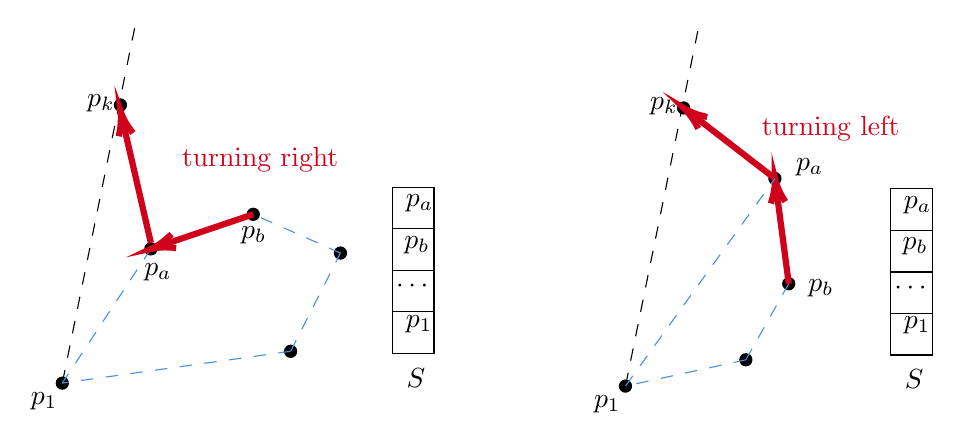
\begin{tikzpicture}[x=0.5pt,y=0.5pt,yscale=-1,xscale=1]
%uncomment if require: \path (0,384); %set diagram left start at 0, and has height of 384

%Flowchart: Connector [id:dp3291568735294871] 
\draw  [fill={rgb, 255:red, 0; green, 0; blue, 0 }  ,fill opacity=1 ] (78,116) .. controls (78,113.58) and (79.96,111.62) .. (82.38,111.62) .. controls (84.79,111.62) and (86.75,113.58) .. (86.75,116) .. controls (86.75,118.42) and (84.79,120.38) .. (82.38,120.38) .. controls (79.96,120.38) and (78,118.42) .. (78,116) -- cycle ;
%Flowchart: Connector [id:dp6621594719883535] 
\draw  [fill={rgb, 255:red, 0; green, 0; blue, 0 }  ,fill opacity=1 ] (201,294) .. controls (201,291.58) and (202.96,289.62) .. (205.38,289.62) .. controls (207.79,289.62) and (209.75,291.58) .. (209.75,294) .. controls (209.75,296.42) and (207.79,298.38) .. (205.38,298.38) .. controls (202.96,298.38) and (201,296.42) .. (201,294) -- cycle ;
%Flowchart: Connector [id:dp25920829224973985] 
\draw  [fill={rgb, 255:red, 0; green, 0; blue, 0 }  ,fill opacity=1 ] (36,317) .. controls (36,314.58) and (37.96,312.62) .. (40.38,312.62) .. controls (42.79,312.62) and (44.75,314.58) .. (44.75,317) .. controls (44.75,319.42) and (42.79,321.38) .. (40.38,321.38) .. controls (37.96,321.38) and (36,319.42) .. (36,317) -- cycle ;
%Flowchart: Connector [id:dp23175126343110752] 
\draw  [fill={rgb, 255:red, 0; green, 0; blue, 0 }  ,fill opacity=1 ] (100,220) .. controls (100,217.58) and (101.96,215.62) .. (104.38,215.62) .. controls (106.79,215.62) and (108.75,217.58) .. (108.75,220) .. controls (108.75,222.42) and (106.79,224.38) .. (104.38,224.38) .. controls (101.96,224.38) and (100,222.42) .. (100,220) -- cycle ;
%Flowchart: Connector [id:dp226256241933963] 
\draw  [fill={rgb, 255:red, 0; green, 0; blue, 0 }  ,fill opacity=1 ] (237,223) .. controls (237,220.58) and (238.96,218.62) .. (241.38,218.62) .. controls (243.79,218.62) and (245.75,220.58) .. (245.75,223) .. controls (245.75,225.42) and (243.79,227.38) .. (241.38,227.38) .. controls (238.96,227.38) and (237,225.42) .. (237,223) -- cycle ;
%Straight Lines [id:da8400967027516107] 
\draw [color={rgb, 255:red, 74; green, 144; blue, 226 }  ,draw opacity=1 ] [dash pattern={on 4.5pt off 4.5pt}]  (205.38,294) -- (40.38,317) ;
%Straight Lines [id:da44754220202255635] 
\draw  [dash pattern={on 4.5pt off 4.5pt}]  (92.63,60.52) -- (40.38,317) ;
%Flowchart: Connector [id:dp1733314058116755] 
\draw  [fill={rgb, 255:red, 0; green, 0; blue, 0 }  ,fill opacity=1 ] (174,195) .. controls (174,192.58) and (175.96,190.62) .. (178.38,190.62) .. controls (180.79,190.62) and (182.75,192.58) .. (182.75,195) .. controls (182.75,197.42) and (180.79,199.38) .. (178.38,199.38) .. controls (175.96,199.38) and (174,197.42) .. (174,195) -- cycle ;
%Straight Lines [id:da6595200138207884] 
\draw [color={rgb, 255:red, 74; green, 144; blue, 226 }  ,draw opacity=1 ] [dash pattern={on 4.5pt off 4.5pt}]  (104.38,220) -- (40.38,317) ;
%Straight Lines [id:da7758013938241641] 
\draw [color={rgb, 255:red, 208; green, 2; blue, 27 }  ,draw opacity=1 ] [dash pattern={on 4.5pt off 4.5pt}]  (178.38,195) -- (104.38,220) ;
%Straight Lines [id:da3686871889066282] 
\draw [color={rgb, 255:red, 74; green, 144; blue, 226 }  ,draw opacity=1 ] [dash pattern={on 4.5pt off 4.5pt}]  (241.38,223) -- (178.38,195) ;
%Straight Lines [id:da610731396524822] 
\draw [color={rgb, 255:red, 74; green, 144; blue, 226 }  ,draw opacity=1 ] [dash pattern={on 4.5pt off 4.5pt}]  (205.38,294) -- (241.38,223) ;
%Shape: Grid [id:dp4209096809685794] 
\draw  [draw opacity=0] (279,175.52) -- (309,175.52) -- (309,295.52) -- (279,295.52) -- cycle ; \draw    ; \draw   (279,205.52) -- (309,205.52)(279,235.52) -- (309,235.52)(279,265.52) -- (309,265.52) ; \draw   (279,175.52) -- (309,175.52) -- (309,295.52) -- (279,295.52) -- cycle ;
%Straight Lines [id:da9339984766179712] 
\draw [color={rgb, 255:red, 208; green, 2; blue, 27 }  ,draw opacity=1 ][line width=2.25]    (104.38,215.62) -- (83.28,124.27) ;
\draw [shift={(82.38,120.38)}, rotate = 436.99] [color={rgb, 255:red, 208; green, 2; blue, 27 }  ,draw opacity=1 ][line width=2.25]    (17.49,-5.26) .. controls (11.12,-2.23) and (5.29,-0.48) .. (0,0) .. controls (5.29,0.48) and (11.12,2.23) .. (17.49,5.26)   ;
%Straight Lines [id:da3526208773719812] 
\draw [color={rgb, 255:red, 208; green, 2; blue, 27 }  ,draw opacity=1 ][line width=2.25]    (178.38,195) -- (108.17,218.72) ;
\draw [shift={(104.38,220)}, rotate = 341.33000000000004] [color={rgb, 255:red, 208; green, 2; blue, 27 }  ,draw opacity=1 ][line width=2.25]    (17.49,-5.26) .. controls (11.12,-2.23) and (5.29,-0.48) .. (0,0) .. controls (5.29,0.48) and (11.12,2.23) .. (17.49,5.26)   ;
%Flowchart: Connector [id:dp777655020217685] 
\draw  [fill={rgb, 255:red, 0; green, 0; blue, 0 }  ,fill opacity=1 ] (485,118.15) .. controls (485,115.73) and (486.96,113.77) .. (489.38,113.77) .. controls (491.79,113.77) and (493.75,115.73) .. (493.75,118.15) .. controls (493.75,120.56) and (491.79,122.52) .. (489.38,122.52) .. controls (486.96,122.52) and (485,120.56) .. (485,118.15) -- cycle ;
%Flowchart: Connector [id:dp9509940585964177] 
\draw  [fill={rgb, 255:red, 0; green, 0; blue, 0 }  ,fill opacity=1 ] (530,300.15) .. controls (530,297.73) and (531.96,295.77) .. (534.38,295.77) .. controls (536.79,295.77) and (538.75,297.73) .. (538.75,300.15) .. controls (538.75,302.56) and (536.79,304.52) .. (534.38,304.52) .. controls (531.96,304.52) and (530,302.56) .. (530,300.15) -- cycle ;
%Flowchart: Connector [id:dp13535258001392825] 
\draw  [fill={rgb, 255:red, 0; green, 0; blue, 0 }  ,fill opacity=1 ] (443,319.15) .. controls (443,316.73) and (444.96,314.77) .. (447.38,314.77) .. controls (449.79,314.77) and (451.75,316.73) .. (451.75,319.15) .. controls (451.75,321.56) and (449.79,323.52) .. (447.38,323.52) .. controls (444.96,323.52) and (443,321.56) .. (443,319.15) -- cycle ;
%Flowchart: Connector [id:dp01259787733434159] 
\draw  [fill={rgb, 255:red, 0; green, 0; blue, 0 }  ,fill opacity=1 ] (551,169.15) .. controls (551,166.73) and (552.96,164.77) .. (555.38,164.77) .. controls (557.79,164.77) and (559.75,166.73) .. (559.75,169.15) .. controls (559.75,171.56) and (557.79,173.52) .. (555.38,173.52) .. controls (552.96,173.52) and (551,171.56) .. (551,169.15) -- cycle ;
%Straight Lines [id:da6618567782842074] 
\draw [color={rgb, 255:red, 74; green, 144; blue, 226 }  ,draw opacity=1 ] [dash pattern={on 4.5pt off 4.5pt}]  (534.38,300.15) -- (447.38,319.15) ;
%Straight Lines [id:da16840703639725407] 
\draw  [dash pattern={on 4.5pt off 4.5pt}]  (499.63,62.67) -- (447.38,319.15) ;
%Flowchart: Connector [id:dp28567136793902825] 
\draw  [fill={rgb, 255:red, 0; green, 0; blue, 0 }  ,fill opacity=1 ] (561,245.15) .. controls (561,242.73) and (562.96,240.77) .. (565.38,240.77) .. controls (567.79,240.77) and (569.75,242.73) .. (569.75,245.15) .. controls (569.75,247.56) and (567.79,249.52) .. (565.38,249.52) .. controls (562.96,249.52) and (561,247.56) .. (561,245.15) -- cycle ;
%Straight Lines [id:da795218588512217] 
\draw [color={rgb, 255:red, 74; green, 144; blue, 226 }  ,draw opacity=1 ] [dash pattern={on 4.5pt off 4.5pt}]  (555.38,169.15) -- (565.38,240.77) ;
%Straight Lines [id:da8869217620231401] 
\draw [color={rgb, 255:red, 74; green, 144; blue, 226 }  ,draw opacity=1 ] [dash pattern={on 4.5pt off 4.5pt}]  (534.38,300.15) -- (565.38,245.15) ;
%Shape: Grid [id:dp22696195921051476] 
\draw  [draw opacity=0] (639,176.67) -- (669,176.67) -- (669,296.67) -- (639,296.67) -- cycle ; \draw    ; \draw   (639,206.67) -- (669,206.67)(639,236.67) -- (669,236.67)(639,266.67) -- (669,266.67) ; \draw   (639,176.67) -- (669,176.67) -- (669,296.67) -- (639,296.67) -- cycle ;
%Straight Lines [id:da10377189210248139] 
\draw [color={rgb, 255:red, 208; green, 2; blue, 27 }  ,draw opacity=1 ][line width=2.25]    (565.38,245.15) -- (555.9,173.11) ;
\draw [shift={(555.38,169.15)}, rotate = 442.5] [color={rgb, 255:red, 208; green, 2; blue, 27 }  ,draw opacity=1 ][line width=2.25]    (17.49,-5.26) .. controls (11.12,-2.23) and (5.29,-0.48) .. (0,0) .. controls (5.29,0.48) and (11.12,2.23) .. (17.49,5.26)   ;
%Straight Lines [id:da44393308824629707] 
\draw [color={rgb, 255:red, 208; green, 2; blue, 27 }  ,draw opacity=1 ][line width=2.25]    (555.38,169.15) -- (492.54,120.59) ;
\draw [shift={(489.38,118.15)}, rotate = 397.69] [color={rgb, 255:red, 208; green, 2; blue, 27 }  ,draw opacity=1 ][line width=2.25]    (17.49,-5.26) .. controls (11.12,-2.23) and (5.29,-0.48) .. (0,0) .. controls (5.29,0.48) and (11.12,2.23) .. (17.49,5.26)   ;
%Straight Lines [id:da7079759298622591] 
\draw [color={rgb, 255:red, 74; green, 144; blue, 226 }  ,draw opacity=1 ] [dash pattern={on 4.5pt off 4.5pt}]  (447.38,319.15) -- (555.38,169.15) ;

% Text Node
\draw (97.75,228.93) node [anchor=north west][inner sep=0.75pt]   [align=left] {$\displaystyle p_{a}$};
% Text Node
\draw (15.75,321.93) node [anchor=north west][inner sep=0.75pt]   [align=left] {$\displaystyle p_{1}$};
% Text Node
\draw (167.75,201.93) node [anchor=north west][inner sep=0.75pt]   [align=left] {$\displaystyle p_{b}$};
% Text Node
\draw (56.38,106.31) node [anchor=north west][inner sep=0.75pt]   [align=left] {$\displaystyle p_{k}$};
% Text Node
\draw (286.75,178.93) node [anchor=north west][inner sep=0.75pt]   [align=left] {$\displaystyle p_{a}$};
% Text Node
\draw (285.75,208.93) node [anchor=north west][inner sep=0.75pt]   [align=left] {$\displaystyle p_{b}$};
% Text Node
\draw (279.75,240.93) node [anchor=north west][inner sep=0.75pt]   [align=left] {$\displaystyle \cdots $};
% Text Node
\draw (286.75,266.08) node [anchor=north west][inner sep=0.75pt]   [align=left] {$\displaystyle p_{1}$};
% Text Node
\draw (287.38,304.31) node [anchor=north west][inner sep=0.75pt]   [align=left] {$\displaystyle S$};
% Text Node
\draw (125,144.93) node [anchor=north west][inner sep=0.75pt]   [align=left] {\textcolor[rgb]{0.82,0.01,0.11}{turning right}};
% Text Node
\draw (568.75,153.08) node [anchor=north west][inner sep=0.75pt]   [align=left] {$\displaystyle p_{a}$};
% Text Node
\draw (422.75,324.08) node [anchor=north west][inner sep=0.75pt]   [align=left] {$\displaystyle p_{1}$};
% Text Node
\draw (577.75,240.08) node [anchor=north west][inner sep=0.75pt]   [align=left] {$\displaystyle p_{b}$};
% Text Node
\draw (463.38,108.46) node [anchor=north west][inner sep=0.75pt]   [align=left] {$\displaystyle p_{k}$};
% Text Node
\draw (646.75,180.08) node [anchor=north west][inner sep=0.75pt]   [align=left] {$\displaystyle p_{a}$};
% Text Node
\draw (645.75,210.08) node [anchor=north west][inner sep=0.75pt]   [align=left] {$\displaystyle p_{b}$};
% Text Node
\draw (639.75,242.08) node [anchor=north west][inner sep=0.75pt]   [align=left] {$\displaystyle \cdots $};
% Text Node
\draw (646.75,267.23) node [anchor=north west][inner sep=0.75pt]   [align=left] {$\displaystyle p_{1}$};
% Text Node
\draw (647.38,305.46) node [anchor=north west][inner sep=0.75pt]   [align=left] {$\displaystyle S$};
% Text Node
\draw (544,122.08) node [anchor=north west][inner sep=0.75pt]   [align=left] {\textcolor[rgb]{0.82,0.01,0.11}{turning left}};


\end{tikzpicture}

}
\caption{Procedure to decide if top element of $S$ is on $CH(p_1, p_2, \cdots, p_k)$.}
\label{fig:invariant}
\end{figure}


How to guarantee above invariant? Consider the general case when we are processing $p_k$.
Now we know that $S$ stores $CH(p_1, p_2, \cdots, p_{k-1})$, and the goal is to determine $CH(p_1, p_2, \cdots, p_k)$.
Following above Property 2, we know that $CH(p_1, p_2, \cdots, p_k) = CH(CH(p_1, p_2, \cdots, p_{k-1}) \cup \{p_k\})$.
Hence we only need to consider the points in $S$ and the current point $p_k$.

But the issue is that, points in $S$, which is exactly $CH(p_1, p_2, \cdots, p_{k-1}$, may not be in
$CH(p_1, p_2, \cdots, p_k)$.  We therefore need to \emph{determine} and \emph{exclude} such points in $S$.
How? See Figure~\ref{fig:invariant} for an example.
We use the following procedure to determine if the top element, called $p_a$, of $S$ is on 
$CH(p_1, p_2, \cdots, p_k)$: we check the \emph{orientation} of the three points $p_b \to p_a \to p_k$,
where $p_a$ and $p_b$ are the top and second top elements of $S$ respectively.
If it's ``turning right'', then $p_a$ will not be on $CH(p_1, p_2, \cdots, p_k)$.
Why? Because in this case $p_a$ will be within triangle $p_1p_bp_k$~(the angle of $p_a$ is in the middle of that of $p_b$ and $p_k$).
If this happens, we can remove $p_a$ safely, i.e., by calling \emph{pop~($S$)}, as $p_a$ cannot be in the convex hull of the first $k$ points.
After we remove $p_a$ from $S$, we will need to continue to examine the top element of $S$ iteratively.
If the orientation is ``turning left'', then actually we get the convex hull of the first $k$ points---that's the points in $S$ plus $p_k$, where $p_k$ will be 
pushed into $S$ and become the top element of $S$. We will give a formal proof after the algorithm.



The complete Gramham-Scan algorithm is illustrated with pseudo-code below.

\begin{minipage}{0.8\textwidth}
	\aaA {5}{Algorithm Graham-Scan ($P$)}\xxx
	\aab {calculate point $p_*$ in $P$ with smallest $y$-coordinate;}\xxx
	\aab {sort $P$ in ascending order of the angles w.r.t.\ $p_*$ and $(\infty, 0)$;}\xxx
	\aab {rename points in $P$ so that points in $P$ are following above order;}\xxx
	\aab {Graham-Scan-Core ($P$);}\xxx
	\aaa {end algorithm;}\xxx
\end{minipage}

\begin{minipage}{0.8\textwidth}
	\aaA {14}{Algorithm Graham-Scan-Core ($P = \{p_1, p_2, \cdots, p_n\}$)}\xxx
	\aab {init empty stack $S$;}\xxx
	\aab {\emph{push ($S, p_1$)};}\xxx
	\aab {\emph{push ($S, p_2$)};}\xxx
	\aab {\emph{push ($S, p_3$)};}\xxx
	\aaB {8}{for $k = 4$ to $n$}\xxx
	\aaC {5}{while ($S$ is not empty)}\xxx
	\aad {let $p_a$ and $p_b$ be the top two elements of $S$;}\xxx
	\aad {check the orientation of $p_b \to p_a \to p_k$;}\xxx
	\aad {if ``turning right'': \emph{pop ($S$)} and then continue the while loop;}\xxx
	\aad {if ``turning left'': break the while loop;}\xxx
	\aac {end while;}\xxx
	\aac {\emph{push ($S, p_k$)};}\xxx
	\aab {end for;}\xxx
	\aaa {end algorithm;}\xxx
\end{minipage}

%%Second, notice that $p_k$ must be on $CH(p_1, p_2, \cdots, p_k)$. Why?
%%This can be proved using line $p_1p_k$ following Property 1: line $p_1p_k$ goes through point $p_k$
%%and all others points in $S$ are on the right side of this line~(this is because points in $P$ are sorted
%%and we are processing them in counter-clockwise order; you can see now the reason why we sort points
%%in this way).


Now we show that, when the while-loop breaks, i.e., the orientation is ``turning left'', then  
$S\cup \{p_k\}$ becomes the convex hull of $\{p_1, p_2, \cdots, p_k\}$.
The proof is based on the definition of convex-hull: we will verify that $S\cup \{p_k\}$ is the smallest, convex polygon that includes all $\{p_1, p_2, \cdots, p_k\}$.
First, we verify that $S\cup \{p_k\}$ forms a convex polygon. This is because, all consecutive 3 points of $S$ are ``turning left'', as this is guaranteed by the algorithm: 
we push $p_k$ right after verifying $p_b\to p_a\to p_k$ are turning left.
To verify that it is circularly ``turning left'', we further need to show that two more consecutive 3 points, namely, $(p_a, p_k, p_1)$ and $(p_k, p_1, p_2)$,
are also turning left.  These are easy to see as $p_kp_1$ are the rightmost line and all other points, including $p_1$ and $p_a$ are on the right side of this line.
Second, we verify that the convex polygon formed by $S\cup \{p_k\}$ contains all points in $\{p_1,p_2,\cdots, p_k\}$.
To see this, we just need to show that all poped points are not possible to be in $CH(p_1, p_2, \cdots, p_k)$,
and this is true, as every poped point is inside of a triangle~(Figure~\ref{fig:invariant}), and therefore must be inside of the convex hull. %$CH(p_1, p_2, \cdots, p_k)$.
Third, we show that $S\cup \{p_k\}$ is the smallest convex polygon that include all first $k$ points.
This is obvious as $S\cup \{p_k\}$ is a subset of the first $k$ points.


\begin{figure}[h!]
\centering{

\tikzset{every picture/.style={line width=0.75pt}} %set default line width to 0.75pt        

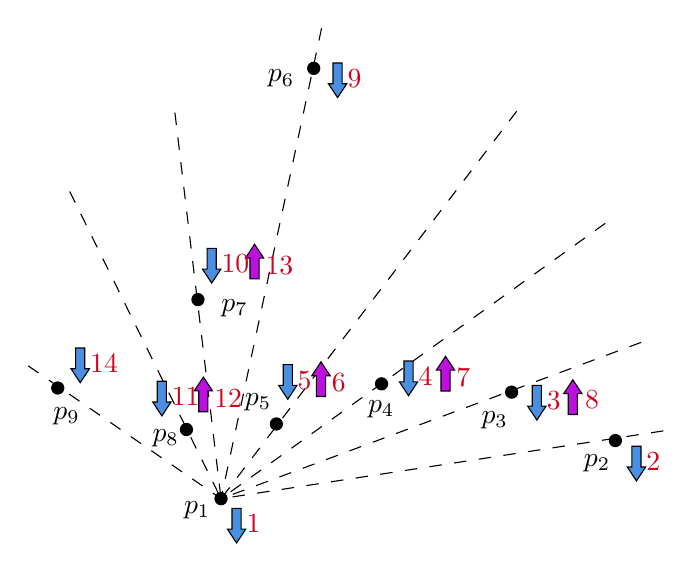
\begin{tikzpicture}[x=0.5pt,y=0.5pt,yscale=-1,xscale=1]
%uncomment if require: \path (0,384); %set diagram left start at 0, and has height of 384

%Flowchart: Connector [id:dp05090347480351787] 
\draw  [fill={rgb, 255:red, 0; green, 0; blue, 0 }  ,fill opacity=1 ] (6,263) .. controls (6,260.58) and (7.96,258.62) .. (10.38,258.62) .. controls (12.79,258.62) and (14.75,260.58) .. (14.75,263) .. controls (14.75,265.42) and (12.79,267.38) .. (10.38,267.38) .. controls (7.96,267.38) and (6,265.42) .. (6,263) -- cycle ;
%Flowchart: Connector [id:dp3291568735294871] 
\draw  [fill={rgb, 255:red, 0; green, 0; blue, 0 }  ,fill opacity=1 ] (191,32) .. controls (191,29.58) and (192.96,27.62) .. (195.38,27.62) .. controls (197.79,27.62) and (199.75,29.58) .. (199.75,32) .. controls (199.75,34.42) and (197.79,36.38) .. (195.38,36.38) .. controls (192.96,36.38) and (191,34.42) .. (191,32) -- cycle ;
%Flowchart: Connector [id:dp6621594719883535] 
\draw  [fill={rgb, 255:red, 0; green, 0; blue, 0 }  ,fill opacity=1 ] (409,301) .. controls (409,298.58) and (410.96,296.62) .. (413.38,296.62) .. controls (415.79,296.62) and (417.75,298.58) .. (417.75,301) .. controls (417.75,303.42) and (415.79,305.38) .. (413.38,305.38) .. controls (410.96,305.38) and (409,303.42) .. (409,301) -- cycle ;
%Flowchart: Connector [id:dp25920829224973985] 
\draw  [fill={rgb, 255:red, 0; green, 0; blue, 0 }  ,fill opacity=1 ] (124,343) .. controls (124,340.58) and (125.96,338.62) .. (128.38,338.62) .. controls (130.79,338.62) and (132.75,340.58) .. (132.75,343) .. controls (132.75,345.42) and (130.79,347.38) .. (128.38,347.38) .. controls (125.96,347.38) and (124,345.42) .. (124,343) -- cycle ;
%Flowchart: Connector [id:dp02220382507011076] 
\draw  [fill={rgb, 255:red, 0; green, 0; blue, 0 }  ,fill opacity=1 ] (107.33,199.13) .. controls (107.33,196.71) and (109.29,194.75) .. (111.71,194.75) .. controls (114.12,194.75) and (116.08,196.71) .. (116.08,199.13) .. controls (116.08,201.54) and (114.12,203.5) .. (111.71,203.5) .. controls (109.29,203.5) and (107.33,201.54) .. (107.33,199.13) -- cycle ;
%Flowchart: Connector [id:dp23175126343110752] 
\draw  [fill={rgb, 255:red, 0; green, 0; blue, 0 }  ,fill opacity=1 ] (164,289) .. controls (164,286.58) and (165.96,284.62) .. (168.38,284.62) .. controls (170.79,284.62) and (172.75,286.58) .. (172.75,289) .. controls (172.75,291.42) and (170.79,293.38) .. (168.38,293.38) .. controls (165.96,293.38) and (164,291.42) .. (164,289) -- cycle ;
%Flowchart: Connector [id:dp17094843613555022] 
\draw  [fill={rgb, 255:red, 0; green, 0; blue, 0 }  ,fill opacity=1 ] (99,293) .. controls (99,290.58) and (100.96,288.62) .. (103.38,288.62) .. controls (105.79,288.62) and (107.75,290.58) .. (107.75,293) .. controls (107.75,295.42) and (105.79,297.38) .. (103.38,297.38) .. controls (100.96,297.38) and (99,295.42) .. (99,293) -- cycle ;
%Flowchart: Connector [id:dp226256241933963] 
\draw  [fill={rgb, 255:red, 0; green, 0; blue, 0 }  ,fill opacity=1 ] (334,266) .. controls (334,263.58) and (335.96,261.62) .. (338.38,261.62) .. controls (340.79,261.62) and (342.75,263.58) .. (342.75,266) .. controls (342.75,268.42) and (340.79,270.38) .. (338.38,270.38) .. controls (335.96,270.38) and (334,268.42) .. (334,266) -- cycle ;
%Straight Lines [id:da8400967027516107] 
\draw  [dash pattern={on 4.5pt off 4.5pt}]  (448.04,294) -- (128.38,343) ;
%Straight Lines [id:da35176427780376085] 
\draw  [dash pattern={on 4.5pt off 4.5pt}]  (432.04,230) -- (128.38,343) ;
%Straight Lines [id:da44754220202255635] 
\draw  [dash pattern={on 4.5pt off 4.5pt}]  (201.04,3) -- (128.38,343) ;
%Straight Lines [id:da6411291076726345] 
\draw  [dash pattern={on 4.5pt off 4.5pt}]  (406.04,144) -- (128.38,343) ;
%Straight Lines [id:da7765810667431168] 
\draw  [dash pattern={on 4.5pt off 4.5pt}]  (342.04,63) -- (128.38,343) ;
%Straight Lines [id:da25629499567852587] 
\draw  [dash pattern={on 4.5pt off 4.5pt}]  (19.04,121) -- (128.38,343) ;
%Straight Lines [id:da38301578845287143] 
\draw  [dash pattern={on 4.5pt off 4.5pt}]  (95.04,64) -- (128.38,343) ;
%Straight Lines [id:da16640897796311926] 
\draw  [dash pattern={on 4.5pt off 4.5pt}]  (-10.96,247) -- (128.38,343) ;
%Flowchart: Connector [id:dp1733314058116755] 
\draw  [fill={rgb, 255:red, 0; green, 0; blue, 0 }  ,fill opacity=1 ] (240,260) .. controls (240,257.58) and (241.96,255.62) .. (244.38,255.62) .. controls (246.79,255.62) and (248.75,257.58) .. (248.75,260) .. controls (248.75,262.42) and (246.79,264.38) .. (244.38,264.38) .. controls (241.96,264.38) and (240,262.42) .. (240,260) -- cycle ;
%Down Arrow [id:dp5063296890502299] 
\draw  [fill={rgb, 255:red, 74; green, 144; blue, 226 }  ,fill opacity=1 ] (133,364.98) -- (136.31,364.98) -- (136.31,349.96) -- (142.92,349.96) -- (142.92,364.98) -- (146.23,364.98) -- (139.62,375) -- cycle ;
%Down Arrow [id:dp21678159444166145] 
\draw  [fill={rgb, 255:red, 74; green, 144; blue, 226 }  ,fill opacity=1 ] (350,276.13) -- (353.31,276.13) -- (353.31,261.11) -- (359.92,261.11) -- (359.92,276.13) -- (363.23,276.13) -- (356.62,286.15) -- cycle ;
%Down Arrow [id:dp6650103756429173] 
\draw  [fill={rgb, 255:red, 74; green, 144; blue, 226 }  ,fill opacity=1 ] (422,320.13) -- (425.31,320.13) -- (425.31,305.11) -- (431.92,305.11) -- (431.92,320.13) -- (435.23,320.13) -- (428.62,330.15) -- cycle ;
%Down Arrow [id:dp802092939622919] 
\draw  [fill={rgb, 255:red, 74; green, 144; blue, 226 }  ,fill opacity=1 ] (257.28,258.53) -- (260.59,258.53) -- (260.59,243.5) -- (267.21,243.5) -- (267.21,258.53) -- (270.51,258.53) -- (263.9,268.54) -- cycle ;
%Down Arrow [id:dp347678952148445] 
\draw  [fill={rgb, 255:red, 74; green, 144; blue, 226 }  ,fill opacity=1 ] (170,261.13) -- (173.31,261.13) -- (173.31,246.11) -- (179.92,246.11) -- (179.92,261.13) -- (183.23,261.13) -- (176.62,271.15) -- cycle ;
%Down Arrow [id:dp2571168081440359] 
\draw  [fill={rgb, 255:red, 74; green, 144; blue, 226 }  ,fill opacity=1 ] (206,43.13) -- (209.31,43.13) -- (209.31,28.11) -- (215.92,28.11) -- (215.92,43.13) -- (219.23,43.13) -- (212.62,53.15) -- cycle ;
%Down Arrow [id:dp43517140651566777] 
\draw  [fill={rgb, 255:red, 74; green, 144; blue, 226 }  ,fill opacity=1 ] (115,177.13) -- (118.31,177.13) -- (118.31,162.11) -- (124.92,162.11) -- (124.92,177.13) -- (128.23,177.13) -- (121.62,187.15) -- cycle ;
%Down Arrow [id:dp31131733900650227] 
\draw  [fill={rgb, 255:red, 74; green, 144; blue, 226 }  ,fill opacity=1 ] (79,273.13) -- (82.31,273.13) -- (82.31,258.11) -- (88.92,258.11) -- (88.92,273.13) -- (92.23,273.13) -- (85.62,283.15) -- cycle ;
%Down Arrow [id:dp9776785564723787] 
\draw  [fill={rgb, 255:red, 74; green, 144; blue, 226 }  ,fill opacity=1 ] (20,249.13) -- (23.31,249.13) -- (23.31,234.11) -- (29.92,234.11) -- (29.92,249.13) -- (33.23,249.13) -- (26.62,259.15) -- cycle ;
%Down Arrow [id:dp6804288828832812] 
\draw  [fill={rgb, 255:red, 189; green, 16; blue, 224 }  ,fill opacity=1 ] (207.23,254.12) -- (203.92,254.12) -- (203.92,269.15) -- (197.31,269.15) -- (197.31,254.12) -- (194,254.12) -- (200.62,244.11) -- cycle ;
%Down Arrow [id:dp2744672671561321] 
\draw  [fill={rgb, 255:red, 189; green, 16; blue, 224 }  ,fill opacity=1 ] (297.23,250.12) -- (293.92,250.12) -- (293.92,265.15) -- (287.31,265.15) -- (287.31,250.12) -- (284,250.12) -- (290.62,240.11) -- cycle ;
%Down Arrow [id:dp749364135043204] 
\draw  [fill={rgb, 255:red, 189; green, 16; blue, 224 }  ,fill opacity=1 ] (389.23,267.12) -- (385.92,267.12) -- (385.92,282.15) -- (379.31,282.15) -- (379.31,267.12) -- (376,267.12) -- (382.62,257.11) -- cycle ;
%Down Arrow [id:dp4501075590171838] 
\draw  [fill={rgb, 255:red, 189; green, 16; blue, 224 }  ,fill opacity=1 ] (159.23,169.12) -- (155.92,169.12) -- (155.92,184.15) -- (149.31,184.15) -- (149.31,169.12) -- (146,169.12) -- (152.62,159.11) -- cycle ;
%Down Arrow [id:dp720924322469968] 
\draw  [fill={rgb, 255:red, 189; green, 16; blue, 224 }  ,fill opacity=1 ] (122.23,265.12) -- (118.92,265.12) -- (118.92,280.15) -- (112.31,280.15) -- (112.31,265.12) -- (109,265.12) -- (115.62,255.11) -- cycle ;

% Text Node
\draw (77,290.93) node [anchor=north west][inner sep=0.75pt]   [align=left] {$\displaystyle p_{8}$};
% Text Node
\draw (126.75,196.93) node [anchor=north west][inner sep=0.75pt]   [align=left] {$\displaystyle p_{7}$};
% Text Node
\draw (143.75,264.93) node [anchor=north west][inner sep=0.75pt]   [align=left] {$\displaystyle p_{5}$};
% Text Node
\draw (232.75,269.93) node [anchor=north west][inner sep=0.75pt]   [align=left] {$\displaystyle p_{4}$};
% Text Node
\draw (99.75,342.93) node [anchor=north west][inner sep=0.75pt]   [align=left] {$\displaystyle p_{1}$};
% Text Node
\draw (388.75,308.93) node [anchor=north west][inner sep=0.75pt]   [align=left] {$\displaystyle p_{2}$};
% Text Node
\draw (5.38,275.31) node [anchor=north west][inner sep=0.75pt]   [align=left] {$\displaystyle p_{9}$};
% Text Node
\draw (160.38,31.31) node [anchor=north west][inner sep=0.75pt]   [align=left] {$\displaystyle p_{6}$};
% Text Node
\draw (314.75,277.93) node [anchor=north west][inner sep=0.75pt]   [align=left] {$\displaystyle p_{3}$};
% Text Node
\draw (144.92,352.89) node [anchor=north west][inner sep=0.75pt]   [align=left] {\textcolor[rgb]{0.82,0.01,0.11}{1}};
% Text Node
\draw (433.92,308.04) node [anchor=north west][inner sep=0.75pt]   [align=left] {$\displaystyle \textcolor[rgb]{0.82,0.01,0.11}{2}$};
% Text Node
\draw (361.92,264.04) node [anchor=north west][inner sep=0.75pt]   [align=left] {$\displaystyle \textcolor[rgb]{0.82,0.01,0.11}{3}$};
% Text Node
\draw (269.21,246.44) node [anchor=north west][inner sep=0.75pt]   [align=left] {$\displaystyle \textcolor[rgb]{0.82,0.01,0.11}{4}$};
% Text Node
\draw (181.92,249.04) node [anchor=north west][inner sep=0.75pt]   [align=left] {$\displaystyle \textcolor[rgb]{0.82,0.01,0.11}{5}$};
% Text Node
\draw (217.92,31.04) node [anchor=north west][inner sep=0.75pt]   [align=left] {$\displaystyle \textcolor[rgb]{0.82,0.01,0.11}{9}$};
% Text Node
\draw (206.62,251.04) node [anchor=north west][inner sep=0.75pt]   [align=left] {$\displaystyle \textcolor[rgb]{0.82,0.01,0.11}{6}$};
% Text Node
\draw (296.62,247.04) node [anchor=north west][inner sep=0.75pt]   [align=left] {$\displaystyle \textcolor[rgb]{0.82,0.01,0.11}{7}$};
% Text Node
\draw (389.62,263.04) node [anchor=north west][inner sep=0.75pt]   [align=left] {$\displaystyle \textcolor[rgb]{0.82,0.01,0.11}{8}$};
% Text Node
\draw (158.62,166.04) node [anchor=north west][inner sep=0.75pt]   [align=left] {$\displaystyle \textcolor[rgb]{0.82,0.01,0.11}{13}$};
% Text Node
\draw (90.92,261.04) node [anchor=north west][inner sep=0.75pt]   [align=left] {$\displaystyle \textcolor[rgb]{0.82,0.01,0.11}{11}$};
% Text Node
\draw (121.62,262.04) node [anchor=north west][inner sep=0.75pt]   [align=left] {$\displaystyle \textcolor[rgb]{0.82,0.01,0.11}{12}$};
% Text Node
\draw (126.92,165.04) node [anchor=north west][inner sep=0.75pt]   [align=left] {$\displaystyle \textcolor[rgb]{0.82,0.01,0.11}{10}$};
% Text Node
\draw (31.92,237.04) node [anchor=north west][inner sep=0.75pt]   [align=left] {$\displaystyle \textcolor[rgb]{0.82,0.01,0.11}{14}$};


\end{tikzpicture}

}
\caption{Running Graham-Scan-Core on the example given in Figure~\ref{fig:sorting}.
Blue and pink arrows show the push and pop operations; the red numbers show
the sequential of these operations.}
\end{figure}


The first 3 lines of Gramham-Scan algorithm corresponds to the preprocessing steps,
which produce a sorted list of points. The main body of the algorithm, referred
to as ``Graham-Scan-Core'' here, gradually construct the convex hull and guarantees
above invariant. When the algorithm terminates, the convex hull of all points
are stored in stack $S$.

Graham-Scan-Core can be regarded as an independent algorithm~(you will find its use
in the divide-and-conquer algorithm for convex hull). Its input
is a list of points $P$, in which the first point, i.e.\ $p_1$, is the point with smallest $y$-coordinate,
and the following points, i.e.\ $p_2, p_3, \cdots, p_n$, are placed in ascending order
by their angle w.r.t.\ $p_1$ and $(+\infty, p_1.y)$. The output of Graham-Scan-Core
is $CH(P)$ which will be stored in the stack $S$.

There are two technical details in implementing above algorithms.
First, in the preprocessing step, for each point $p_i$ do we really need to calculate the actual angle
of $\angle p_ip_*p_{\infty}$, where $p_{\infty} = (+\infty, p_*.y)$?
No. Notice that the only purpose of calculating these angles is sorting these points.
Therefore, only the relative order matters but not the actual angles.
Hence, we can calculate $\cos(\cdot)$ of the angle and use it to sort,
as $\cos(\cdot)$ is monotone over $[0,\pi]$. Clearly,
$\cos( \angle p_ip_*p_{\infty} ) = \overrightarrow{p_*p_i}\cdot (1, 0) / |\overrightarrow{p_*p_i}|$.

Second, in Graham-Scan-Core, how to determine
the orientation of 3 points~(i.e.\ $p_b \to p_a \to p_k$)? We will use ``right-hand-rule''.
Define two vectors: $\overrightarrow{A} := \overrightarrow{p_bp_a}$ and $\overrightarrow{B} = \overrightarrow{p_ap_k}$.
Let $\overrightarrow{A} = (x_A,y_A)$ and $\overrightarrow{B}= (x_B, y_B)$ be their coordinates,
which can be calculated from the coordinates of $p_b$, $p_a$ and $p_k$.
The right-hand-rule gives that
\begin{displaymath}
\left\{
	\begin{array}{rccl}
		x_Ay_B - x_By_A & > & 0 \quad \textrm{if and only if} & p_b \to p_a \to p_k \textrm{\ ``turning left''} \\
		x_Ay_B - x_By_A & < & 0 \quad \textrm{if and only if} & p_b \to p_a \to p_k \textrm{\ ``turning right''} \\
		x_Ay_B - x_By_A & = & 0 \quad \textrm{if and only if} & p_b, p_a, p_k \textrm{\ ``colinear''} \\
	\end{array}
\right.
\end{displaymath}

\subsection*{Running Time of Graham-Scan}

Although Graham-Scan-Core consists of two nested loop, in fact it runs in linear time!
To see this, consider the types of operations and how many each type of operation
the algorithm needs to do.  There are three types of operations this algorithm does: \emph{push}, \emph{pop}, and \emph{checking-orientation},
and each operation takes $\Theta(1)$ time. Now let's consider the times of each type will need to execute.
First, notice that \#(\emph{push}) $= n$, as each point will be pushed to the stack exactly once.
Second, \#(\emph{pop}) $\le n$, as \#(\emph{push}) $\le$ \#(\emph{pop}) starting from an empty stack~(a point must be pushed into the stack prior to pop).
Third, notice that right after \emph{checking-orientation} it is either a \emph{push} or a \emph{pop} operation~(i.e.,
it's not possible to have two \emph{checking-orientation} operations next to each other).
This implies that \#(\emph{checking-orientation}) $\le$ \#(\emph{push}) + \#(\emph{pop}) $\le 2n$.
Combined, we have that Graham-Scan-Core takes $\Theta(n)$ time.

The preprocessing step of Graham-Scan takes $\Theta(n \log n)$, as it's dominated by the sorting step.
The entire running time of Graham-Scan therefore takes $\Theta(n \log n)$ time.

\subsection*{Divide-and-Conquer Algorithm}

We now design a divide-and-conquer algorithm for convex hull problem.
As usual, we define recursive function, say, CHDC~($P$), which takes
a set of points $P$ as input and returns $CH(P)$, represented
as the list of vertices of the convex polygon in counter-clockwise order.

\begin{minipage}{0.8\textwidth}
	\aaA {5}{function CHDC~($P = \{p_1, p_2, \cdots, p_n\}$)}\xxx
	\aab {if $n \le 3$: resolve this base case and return the convex hull;}\xxx
	\aab {$C_1$ = CHDC~($P[1..n/2]$);}\xxx
	\aab {$C_2$ = CHDC~($P[n/2 + 1..n]$);}\xxx
	\aab {return \textcolor{blue}{combine~($C_1, C_2$)};}\xxx
	\aaa {end algorithm;}\xxx
\end{minipage}

The ``combine'' function in above pseudo-code is missing.
Before design an algorithm for ``combine'', we first make sure that
it suffices to only consider points in $C_1$ and $C_2$. Formally,
we can write $CH(P) = CH(C_1\cup C_2)$. This can be proved using the
Property~2 of convex hull. Intuitively, any point \emph{inside} $C_1$ or $C_2$
with be inside $CH(P)$, and therefore won't be \emph{on} $CH(P)$.

We can use, for example, Graham-Scan to calculate $CH(C_1\cup C_2)$, which takes $\Theta(m\log m)$, where $m = |C_1\cup C_2|$.
Can we do better? Yes. We will design an $\Theta(m)$ time algorithm to calculate $CH(C_1\cup C_2)$.
The idea is to take advantage of that, $C_1$ and $C_2$ are already sorted~(in counter-clockwise order along the polygon),
and then to use Graham-Scan-Core to calculate $CH(C_1\cup C_2)$. Recall that, Graham-Scan-Core is linear-time algorithm for convex hull;
it just requires that all points in its input is sorted in counter-clockwise order w.r.t.\ the first point in its input.


The pseudo-code for combine procedure is given below.
See figure below for explaining.

\begin{minipage}{0.8\textwidth}
	\aaA {14.5}{function combine~($C_1, C_2$)}\xxx
	\aab {find $p_*$ in $C_1\cup C_2$ with smallest $y$-coordinate;}\xxx
	\aab {assume that $p_*\in C_1$; otherwise exchange $C_1$ and $C_2$;}\xxx
	\aab {rewrite $C_1$ into $C_1'$ with circular shifting so that $p_*$ is the first point of $C_1'$; 
		(\emph{Note: now points in $C_1'$ is sorted w.r.t.\ $p_*$ in counter-clockwise order.})}\xxx
	\aab {find $p_S$ in $C_2$ with smallest angle~(i.e., angle $\angle p_S p_* p_\infty$, where $p_\infty = (+\infty, p_*.y)$;}\xxx
	\aab {find $p_L$ in $C_2$ with largest angle~(i.e., angle $\angle p_L p_* p_\infty$, where $p_\infty = (+\infty, p_*.y)$;}\xxx
	\aab {let $C_{2a}$ be the sublist of $C_2$ from $p_S$ to $p_L$ in counter-clockwise order; 
		(\emph{Note: now points in $C_{2a}$ is sorted w.r.t.\ $p_*$ in counter-clockwise order.})}\xxx
	\aab {let $C_{2b}$ be the sublist of $C_2$ from $p_S$ to $p_L$ in clockwise order;
		(\emph{Note: now points in $C_{2b}$ is sorted w.r.t.\ $p_*$ in counter-clockwise order.})}\xxx
	\aab {$C_2' = $ merge-two-sorted-arrays~($C_{2a}, C_{2b}$);
		(\emph{Note: merging is by the angle w.r.t.\ $p_*$ and $p_\infty$; after it points in $C_2'$ is sorted w.r.t.\ $p_*$ in counter-clockwise order.})}\xxx
	\aab {$C' = $ merge-two-sorted-arrays~($C_1', C_2'$);
		(\emph{Note: merging is by the angle w.r.t.\ $p_*$ and $p_\infty$; after it points in $C'$, i.e., points in $C_1\cup C_2$, is sorted w.r.t.\ $p_*$ in counter-clockwise order.})}\xxx
	\aab {return Graham-Core-Scan~($C'$);}\xxx
	\aaa {end algorithm;}\xxx
\end{minipage}



\begin{figure}[h!]
\centering{

\tikzset{every picture/.style={line width=0.75pt}} %set default line width to 0.75pt        

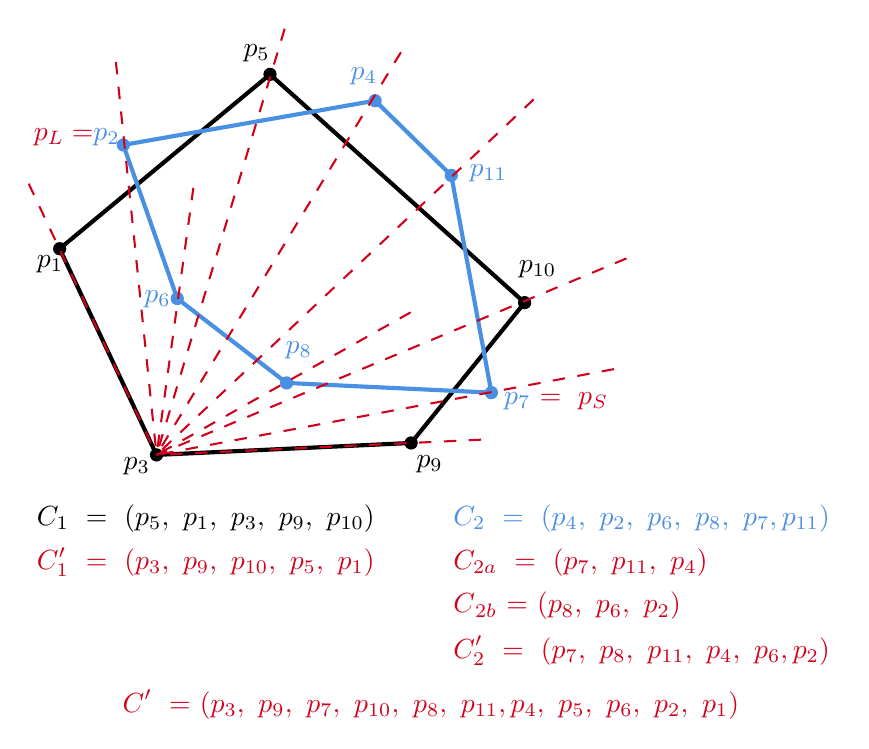
\begin{tikzpicture}[x=0.5pt,y=0.5pt,yscale=-1,xscale=1]
%uncomment if require: \path (0,506); %set diagram left start at 0, and has height of 506

%Flowchart: Connector [id:dp3760201615823463] 
\draw  [fill={rgb, 255:red, 0; green, 0; blue, 0 }  ,fill opacity=1 ] (57,162) .. controls (57,159.58) and (58.96,157.62) .. (61.38,157.62) .. controls (63.79,157.62) and (65.75,159.58) .. (65.75,162) .. controls (65.75,164.42) and (63.79,166.38) .. (61.38,166.38) .. controls (58.96,166.38) and (57,164.42) .. (57,162) -- cycle ;
%Flowchart: Connector [id:dp5854006172506206] 
\draw  [fill={rgb, 255:red, 0; green, 0; blue, 0 }  ,fill opacity=1 ] (209,36) .. controls (209,33.58) and (210.96,31.62) .. (213.38,31.62) .. controls (215.79,31.62) and (217.75,33.58) .. (217.75,36) .. controls (217.75,38.42) and (215.79,40.38) .. (213.38,40.38) .. controls (210.96,40.38) and (209,38.42) .. (209,36) -- cycle ;
%Flowchart: Connector [id:dp03971004338552875] 
\draw  [fill={rgb, 255:red, 0; green, 0; blue, 0 }  ,fill opacity=1 ] (311,302.38) .. controls (311,299.96) and (312.96,298) .. (315.38,298) .. controls (317.79,298) and (319.75,299.96) .. (319.75,302.38) .. controls (319.75,304.79) and (317.79,306.75) .. (315.38,306.75) .. controls (312.96,306.75) and (311,304.79) .. (311,302.38) -- cycle ;
%Flowchart: Connector [id:dp4369716280602779] 
\draw  [fill={rgb, 255:red, 0; green, 0; blue, 0 }  ,fill opacity=1 ] (127,311) .. controls (127,308.58) and (128.96,306.62) .. (131.38,306.62) .. controls (133.79,306.62) and (135.75,308.58) .. (135.75,311) .. controls (135.75,313.42) and (133.79,315.38) .. (131.38,315.38) .. controls (128.96,315.38) and (127,313.42) .. (127,311) -- cycle ;
%Flowchart: Connector [id:dp03888777155399348] 
\draw  [color={rgb, 255:red, 74; green, 144; blue, 226 }  ,draw opacity=1 ][fill={rgb, 255:red, 74; green, 144; blue, 226 }  ,fill opacity=1 ] (103,87) .. controls (103,84.58) and (104.96,82.62) .. (107.38,82.62) .. controls (109.79,82.62) and (111.75,84.58) .. (111.75,87) .. controls (111.75,89.42) and (109.79,91.38) .. (107.38,91.38) .. controls (104.96,91.38) and (103,89.42) .. (103,87) -- cycle ;
%Flowchart: Connector [id:dp6352844555884073] 
\draw  [fill={rgb, 255:red, 0; green, 0; blue, 0 }  ,fill opacity=1 ] (393,201) .. controls (393,198.58) and (394.96,196.62) .. (397.38,196.62) .. controls (399.79,196.62) and (401.75,198.58) .. (401.75,201) .. controls (401.75,203.42) and (399.79,205.38) .. (397.38,205.38) .. controls (394.96,205.38) and (393,203.42) .. (393,201) -- cycle ;
%Flowchart: Connector [id:dp23645115309917453] 
\draw  [color={rgb, 255:red, 74; green, 144; blue, 226 }  ,draw opacity=1 ][fill={rgb, 255:red, 74; green, 144; blue, 226 }  ,fill opacity=1 ] (285,55) .. controls (285,52.58) and (286.96,50.62) .. (289.38,50.62) .. controls (291.79,50.62) and (293.75,52.58) .. (293.75,55) .. controls (293.75,57.42) and (291.79,59.38) .. (289.38,59.38) .. controls (286.96,59.38) and (285,57.42) .. (285,55) -- cycle ;
%Straight Lines [id:da9582823916987413] 
\draw [color={rgb, 255:red, 0; green, 0; blue, 0 }  ,draw opacity=1 ][line width=1.5]    (131.38,311) -- (315.38,302.38) ;
%Straight Lines [id:da7170032735395258] 
\draw [color={rgb, 255:red, 0; green, 0; blue, 0 }  ,draw opacity=1 ][line width=1.5]    (61.38,162) -- (213.38,36) ;
%Straight Lines [id:da7153530187498507] 
\draw [color={rgb, 255:red, 0; green, 0; blue, 0 }  ,draw opacity=1 ][fill={rgb, 255:red, 245; green, 166; blue, 35 }  ,fill opacity=1 ][line width=1.5]    (61.38,162) -- (92.84,228.96) -- (131.38,311) ;
%Straight Lines [id:da6087381521295036] 
\draw [color={rgb, 255:red, 0; green, 0; blue, 0 }  ,draw opacity=1 ][line width=1.5]    (213.38,36) -- (397.38,201) ;
%Straight Lines [id:da7334727922272425] 
\draw [color={rgb, 255:red, 0; green, 0; blue, 0 }  ,draw opacity=1 ][line width=1.5]    (315.38,302.38) -- (397.38,201) ;
%Flowchart: Connector [id:dp3946295929267337] 
\draw  [color={rgb, 255:red, 74; green, 144; blue, 226 }  ,draw opacity=1 ][fill={rgb, 255:red, 74; green, 144; blue, 226 }  ,fill opacity=1 ] (142,198) .. controls (142,195.58) and (143.96,193.62) .. (146.38,193.62) .. controls (148.79,193.62) and (150.75,195.58) .. (150.75,198) .. controls (150.75,200.42) and (148.79,202.38) .. (146.38,202.38) .. controls (143.96,202.38) and (142,200.42) .. (142,198) -- cycle ;
%Flowchart: Connector [id:dp5536782520392832] 
\draw  [color={rgb, 255:red, 74; green, 144; blue, 226 }  ,draw opacity=1 ][fill={rgb, 255:red, 74; green, 144; blue, 226 }  ,fill opacity=1 ] (221,259) .. controls (221,256.58) and (222.96,254.62) .. (225.38,254.62) .. controls (227.79,254.62) and (229.75,256.58) .. (229.75,259) .. controls (229.75,261.42) and (227.79,263.38) .. (225.38,263.38) .. controls (222.96,263.38) and (221,261.42) .. (221,259) -- cycle ;
%Flowchart: Connector [id:dp5354107395187737] 
\draw  [color={rgb, 255:red, 74; green, 144; blue, 226 }  ,draw opacity=1 ][fill={rgb, 255:red, 74; green, 144; blue, 226 }  ,fill opacity=1 ] (369,266) .. controls (369,263.58) and (370.96,261.62) .. (373.38,261.62) .. controls (375.79,261.62) and (377.75,263.58) .. (377.75,266) .. controls (377.75,268.42) and (375.79,270.38) .. (373.38,270.38) .. controls (370.96,270.38) and (369,268.42) .. (369,266) -- cycle ;
%Flowchart: Connector [id:dp21529891001736134] 
\draw  [color={rgb, 255:red, 74; green, 144; blue, 226 }  ,draw opacity=1 ][fill={rgb, 255:red, 74; green, 144; blue, 226 }  ,fill opacity=1 ] (340,109) .. controls (340,106.58) and (341.96,104.62) .. (344.38,104.62) .. controls (346.79,104.62) and (348.75,106.58) .. (348.75,109) .. controls (348.75,111.42) and (346.79,113.38) .. (344.38,113.38) .. controls (341.96,113.38) and (340,111.42) .. (340,109) -- cycle ;
%Straight Lines [id:da13610377148087538] 
\draw [color={rgb, 255:red, 74; green, 144; blue, 226 }  ,draw opacity=1 ][line width=1.5]    (146.38,198) -- (107.38,87) ;
%Straight Lines [id:da17098738082940423] 
\draw [color={rgb, 255:red, 74; green, 144; blue, 226 }  ,draw opacity=1 ][line width=1.5]    (373.38,266) -- (225.38,259) ;
%Straight Lines [id:da39885017452703897] 
\draw [color={rgb, 255:red, 74; green, 144; blue, 226 }  ,draw opacity=1 ][line width=1.5]    (373.38,266) -- (344.38,109) ;
%Straight Lines [id:da49076142701312997] 
\draw [color={rgb, 255:red, 74; green, 144; blue, 226 }  ,draw opacity=1 ][line width=1.5]    (344.38,109) -- (289.38,55) ;
%Straight Lines [id:da7133961892030377] 
\draw [color={rgb, 255:red, 74; green, 144; blue, 226 }  ,draw opacity=1 ][line width=1.5]    (225.38,259) -- (146.38,198) ;
%Straight Lines [id:da6192417354090246] 
\draw [color={rgb, 255:red, 74; green, 144; blue, 226 }  ,draw opacity=1 ][line width=1.5]    (289.38,55) -- (107.38,87) ;
%Straight Lines [id:da3354599107667824] 
\draw [color={rgb, 255:red, 208; green, 2; blue, 27 }  ,draw opacity=1 ][line width=0.75]  [dash pattern={on 4.5pt off 4.5pt}]  (462,249) -- (131.38,311) ;
%Straight Lines [id:da37383354135177016] 
\draw [color={rgb, 255:red, 208; green, 2; blue, 27 }  ,draw opacity=1 ][line width=0.75]  [dash pattern={on 4.5pt off 4.5pt}]  (315,208) -- (131.38,311) ;
%Straight Lines [id:da663432735093426] 
\draw [color={rgb, 255:red, 208; green, 2; blue, 27 }  ,draw opacity=1 ][line width=0.75]  [dash pattern={on 4.5pt off 4.5pt}]  (404,54) -- (131.38,311) ;
%Straight Lines [id:da4154054026142908] 
\draw [color={rgb, 255:red, 208; green, 2; blue, 27 }  ,draw opacity=1 ][line width=0.75]  [dash pattern={on 4.5pt off 4.5pt}]  (308,20) -- (131.38,311) ;
%Straight Lines [id:da9171997534785323] 
\draw [color={rgb, 255:red, 208; green, 2; blue, 27 }  ,draw opacity=1 ][line width=0.75]  [dash pattern={on 4.5pt off 4.5pt}]  (102,27) -- (131.38,311) ;
%Straight Lines [id:da9698007508961525] 
\draw [color={rgb, 255:red, 208; green, 2; blue, 27 }  ,draw opacity=1 ][line width=0.75]  [dash pattern={on 4.5pt off 4.5pt}]  (224,3) -- (131.38,311) ;
%Straight Lines [id:da3710951051522332] 
\draw [color={rgb, 255:red, 208; green, 2; blue, 27 }  ,draw opacity=1 ][line width=0.75]  [dash pattern={on 4.5pt off 4.5pt}]  (158,118) -- (131.38,311) ;
%Straight Lines [id:da8247371840671284] 
\draw [color={rgb, 255:red, 208; green, 2; blue, 27 }  ,draw opacity=1 ][line width=0.75]  [dash pattern={on 4.5pt off 4.5pt}]  (471,169) -- (131.38,311) ;
%Straight Lines [id:da3258545016218505] 
\draw [color={rgb, 255:red, 208; green, 2; blue, 27 }  ,draw opacity=1 ][line width=0.75]  [dash pattern={on 4.5pt off 4.5pt}]  (366,300) -- (131.38,311) ;
%Straight Lines [id:da24778748747353996] 
\draw [color={rgb, 255:red, 208; green, 2; blue, 27 }  ,draw opacity=1 ][line width=0.75]  [dash pattern={on 4.5pt off 4.5pt}]  (39,115) -- (131.38,311) ;

% Text Node
\draw (43,345) node [anchor=north west][inner sep=0.75pt]   [align=left] {$\displaystyle C_{1} \ =\ ( p_{5} ,\ p_{1} ,\ p_{3} ,\ p_{9} ,\ p_{10}) \ $};
% Text Node
\draw (43,165) node [anchor=north west][inner sep=0.75pt]   [align=left] {$\displaystyle p_{1}$};
% Text Node
\draw (40.75,73) node [anchor=north west][inner sep=0.75pt]  [color={rgb, 255:red, 74; green, 144; blue, 226 }  ,opacity=1 ] [align=left] {$\displaystyle \textcolor[rgb]{0.82,0.01,0.11}{p_{L} =} p_{2}$};
% Text Node
\draw (269.75,29) node [anchor=north west][inner sep=0.75pt]  [color={rgb, 255:red, 74; green, 144; blue, 226 }  ,opacity=1 ] [align=left] {$\displaystyle p_{4}$};
% Text Node
\draw (120.75,190) node [anchor=north west][inner sep=0.75pt]  [color={rgb, 255:red, 74; green, 144; blue, 226 }  ,opacity=1 ] [align=left] {$\displaystyle p_{6}$};
% Text Node
\draw (380.75,264) node [anchor=north west][inner sep=0.75pt]  [color={rgb, 255:red, 74; green, 144; blue, 226 }  ,opacity=1 ] [align=left] {$\displaystyle p_{7} \ \textcolor[rgb]{0.82,0.01,0.11}{=\ p_{S}}$};
% Text Node
\draw (105.75,311) node [anchor=north west][inner sep=0.75pt]   [align=left] {$\displaystyle p_{3}$};
% Text Node
\draw (317.38,309.75) node [anchor=north west][inner sep=0.75pt]   [align=left] {$\displaystyle p_{9}$};
% Text Node
\draw (391.38,168.38) node [anchor=north west][inner sep=0.75pt]   [align=left] {$\displaystyle p_{10}$};
% Text Node
\draw (192.38,12.38) node [anchor=north west][inner sep=0.75pt]   [align=left] {$\displaystyle p_{5}$};
% Text Node
\draw (222.75,227) node [anchor=north west][inner sep=0.75pt]  [color={rgb, 255:red, 74; green, 144; blue, 226 }  ,opacity=1 ] [align=left] {$\displaystyle p_{8}$};
% Text Node
\draw (355.75,99) node [anchor=north west][inner sep=0.75pt]  [color={rgb, 255:red, 74; green, 144; blue, 226 }  ,opacity=1 ] [align=left] {$\displaystyle p_{11}$};
% Text Node
\draw (344,345) node [anchor=north west][inner sep=0.75pt]   [align=left] {$\displaystyle \textcolor[rgb]{0.29,0.56,0.89}{C_{2} \ =\ ( p_{4} ,\ p_{2} ,\ p_{6} ,\ p_{8} ,\ p_{7} ,p_{11}) \ }$};
% Text Node
\draw (344,376.67) node [anchor=north west][inner sep=0.75pt]   [align=left] {$\displaystyle \textcolor[rgb]{0.82,0.01,0.11}{C_{2a} \ =\ ( p_{7} ,\ p_{11} ,\ p_{4}) \ }$};
% Text Node
\draw (344,408.34) node [anchor=north west][inner sep=0.75pt]   [align=left] {$\displaystyle \textcolor[rgb]{0.82,0.01,0.11}{C}\textcolor[rgb]{0.82,0.01,0.11}{_{2b}}\textcolor[rgb]{0.82,0.01,0.11}{\ =\ }\textcolor[rgb]{0.82,0.01,0.11}{(}\textcolor[rgb]{0.82,0.01,0.11}{p}\textcolor[rgb]{0.82,0.01,0.11}{_{8}}\textcolor[rgb]{0.82,0.01,0.11}{,\ p}\textcolor[rgb]{0.82,0.01,0.11}{_{6}}\textcolor[rgb]{0.82,0.01,0.11}{,\ p}\textcolor[rgb]{0.82,0.01,0.11}{_{2}}\textcolor[rgb]{0.82,0.01,0.11}{)}\textcolor[rgb]{0.82,0.01,0.11}{\ }$};
% Text Node
\draw (344,440) node [anchor=north west][inner sep=0.75pt]   [align=left] {$\displaystyle \textcolor[rgb]{0.82,0.01,0.11}{C'_{2} \ =\ ( p_{7} ,\ p_{8} ,\ p_{11} ,\ p_{4} ,\ p_{6} ,p_{2}) \ }$};
% Text Node
\draw (43,376) node [anchor=north west][inner sep=0.75pt]   [align=left] {$\displaystyle \textcolor[rgb]{0.82,0.01,0.11}{C'_{1} \ =\ ( p_{3} ,\ p_{9} ,\ p_{10} ,\ p_{5} ,\ p_{1}) \ }$};
% Text Node
\draw (105,479) node [anchor=north west][inner sep=0.75pt]   [align=left] {$\displaystyle \textcolor[rgb]{0.82,0.01,0.11}{C'\ =\ }\textcolor[rgb]{0.82,0.01,0.11}{(}\textcolor[rgb]{0.82,0.01,0.11}{p}\textcolor[rgb]{0.82,0.01,0.11}{_{3}}\textcolor[rgb]{0.82,0.01,0.11}{,\ p}\textcolor[rgb]{0.82,0.01,0.11}{_{9}}\textcolor[rgb]{0.82,0.01,0.11}{,\ p_{7} ,\ p}\textcolor[rgb]{0.82,0.01,0.11}{_{10}}\textcolor[rgb]{0.82,0.01,0.11}{,\ p_{8} ,\ p_{11} ,p_{4} ,\ p}\textcolor[rgb]{0.82,0.01,0.11}{_{5}}\textcolor[rgb]{0.82,0.01,0.11}{,\ p_{6} ,\ p_{2} ,\ p}\textcolor[rgb]{0.82,0.01,0.11}{_{1}}\textcolor[rgb]{0.82,0.01,0.11}{)}\textcolor[rgb]{0.82,0.01,0.11}{\ }$};


\end{tikzpicture}

}
\caption{Example of combining $C_1$ and $C_2$.}
\label{fig:meta-graph}
\end{figure}



Clearly each step of above combine takes linear time. Therefore, the entire running time of combine is $\Theta(|C_1| + |C_2|)$.

To obtain the running time of CHDC, we write its recursion $T(n) = 2T(n/2) + \Theta(|C_1| + |C_2|)$.
In worst case, $|C_1| + |C_2| = \Theta(n)$, and therefore $T(n) = 2T(n/2) + \Theta(n)$, which gives $T(n) = \Theta(n\log n)$.
In this (worst) case the running time of this divide-and-conquer algorithm is the same with Graham-Scan.
However, if the size of $|C_1| + |C_2|$ is in the order of $o(n)$, we will have
improved running time.  For example, if $|C_1| + |C_2| = \Theta(n^{0.99})$, then $T(n) = \Theta(n)$.  
This might happen in practical cases, although in worst case divide-and-conquer runs in $\Theta(n\log n)$ time.
